\chapter{Introduction}
\label{sec:introduction}
%\chapter{Einleitung}
%\label{sec:einleitung}

 One of the major challenges facing the agricultural industry today is the problem of weeds. Traditional methods of weed removal include large amounts of herbicides, which are harmful to the environment, or manual labor, which is extremely time-consuming and tiring. To address this issue, Caterra, a project under the Crop Science Laboratory of ETH Zurich, is developing a robotic system that uses a laser module to automatically eliminate weeds. \\

This project requires the rover robot to navigate autonomously. For now, most agricultural robots use GNSS to accomplish this task. However, GNSS-based navigation is prone to many problems:
\begin{itemize}
    \item It relies on a fixed infrastructure, such as ground-based reference stations, which may not be available or practical in remote agricultural areas.
    \item The field conditions, weather, and other environmental factors can affect the accuracy of the GNSS signals and cause errors in navigation.
    \item The field environment is constantly changing, with crops growing and harvested, making it difficult for the robot to accurately map and navigate the area.
\end{itemize}

In general, GNSS can provide a rough location of the robot in an agricultural field, but it is not the most robust and reliable solution for autonomous navigation. The need for a more robust method with instant feedback is necessary. Machine vision approaches, specifically visual odometry using an RGB camera, have been extensively researched as an alternative. These methods provide greater robustness and precision and are cost-effective and easy to maintain.

The detection of crop rows is a key aspect in enabling proprioception in agricultural robots and can also be used for other important applications such as crop counting, yield prediction, and field mapping. However, due to the variability in crop type, growth stage, and environmental conditions, detecting crop rows is a challenging task. Many image processing techniques that have been developed are often limited in their ability to detect crop rows robustly under different conditions and their need for a significant amount of manual tuning, and there is a pressing need to develop more robust, adaptable, and automated image processing techniques that can effectively handle the variability of crop rows and environmental conditions. \\


To develop such an algorithm, we have integrated three key principles: Hough transform to extract the main lines from the image, vanishing point calculation to eliminate outliers, and RANSAC to obtain more precise information about the center of each crop row while taking into consideration the fundamental characteristics of crop rows. This will enable further research on the autonomous navigation capabilities of the rover robot.

\begin{figure}[H]
   \centering
   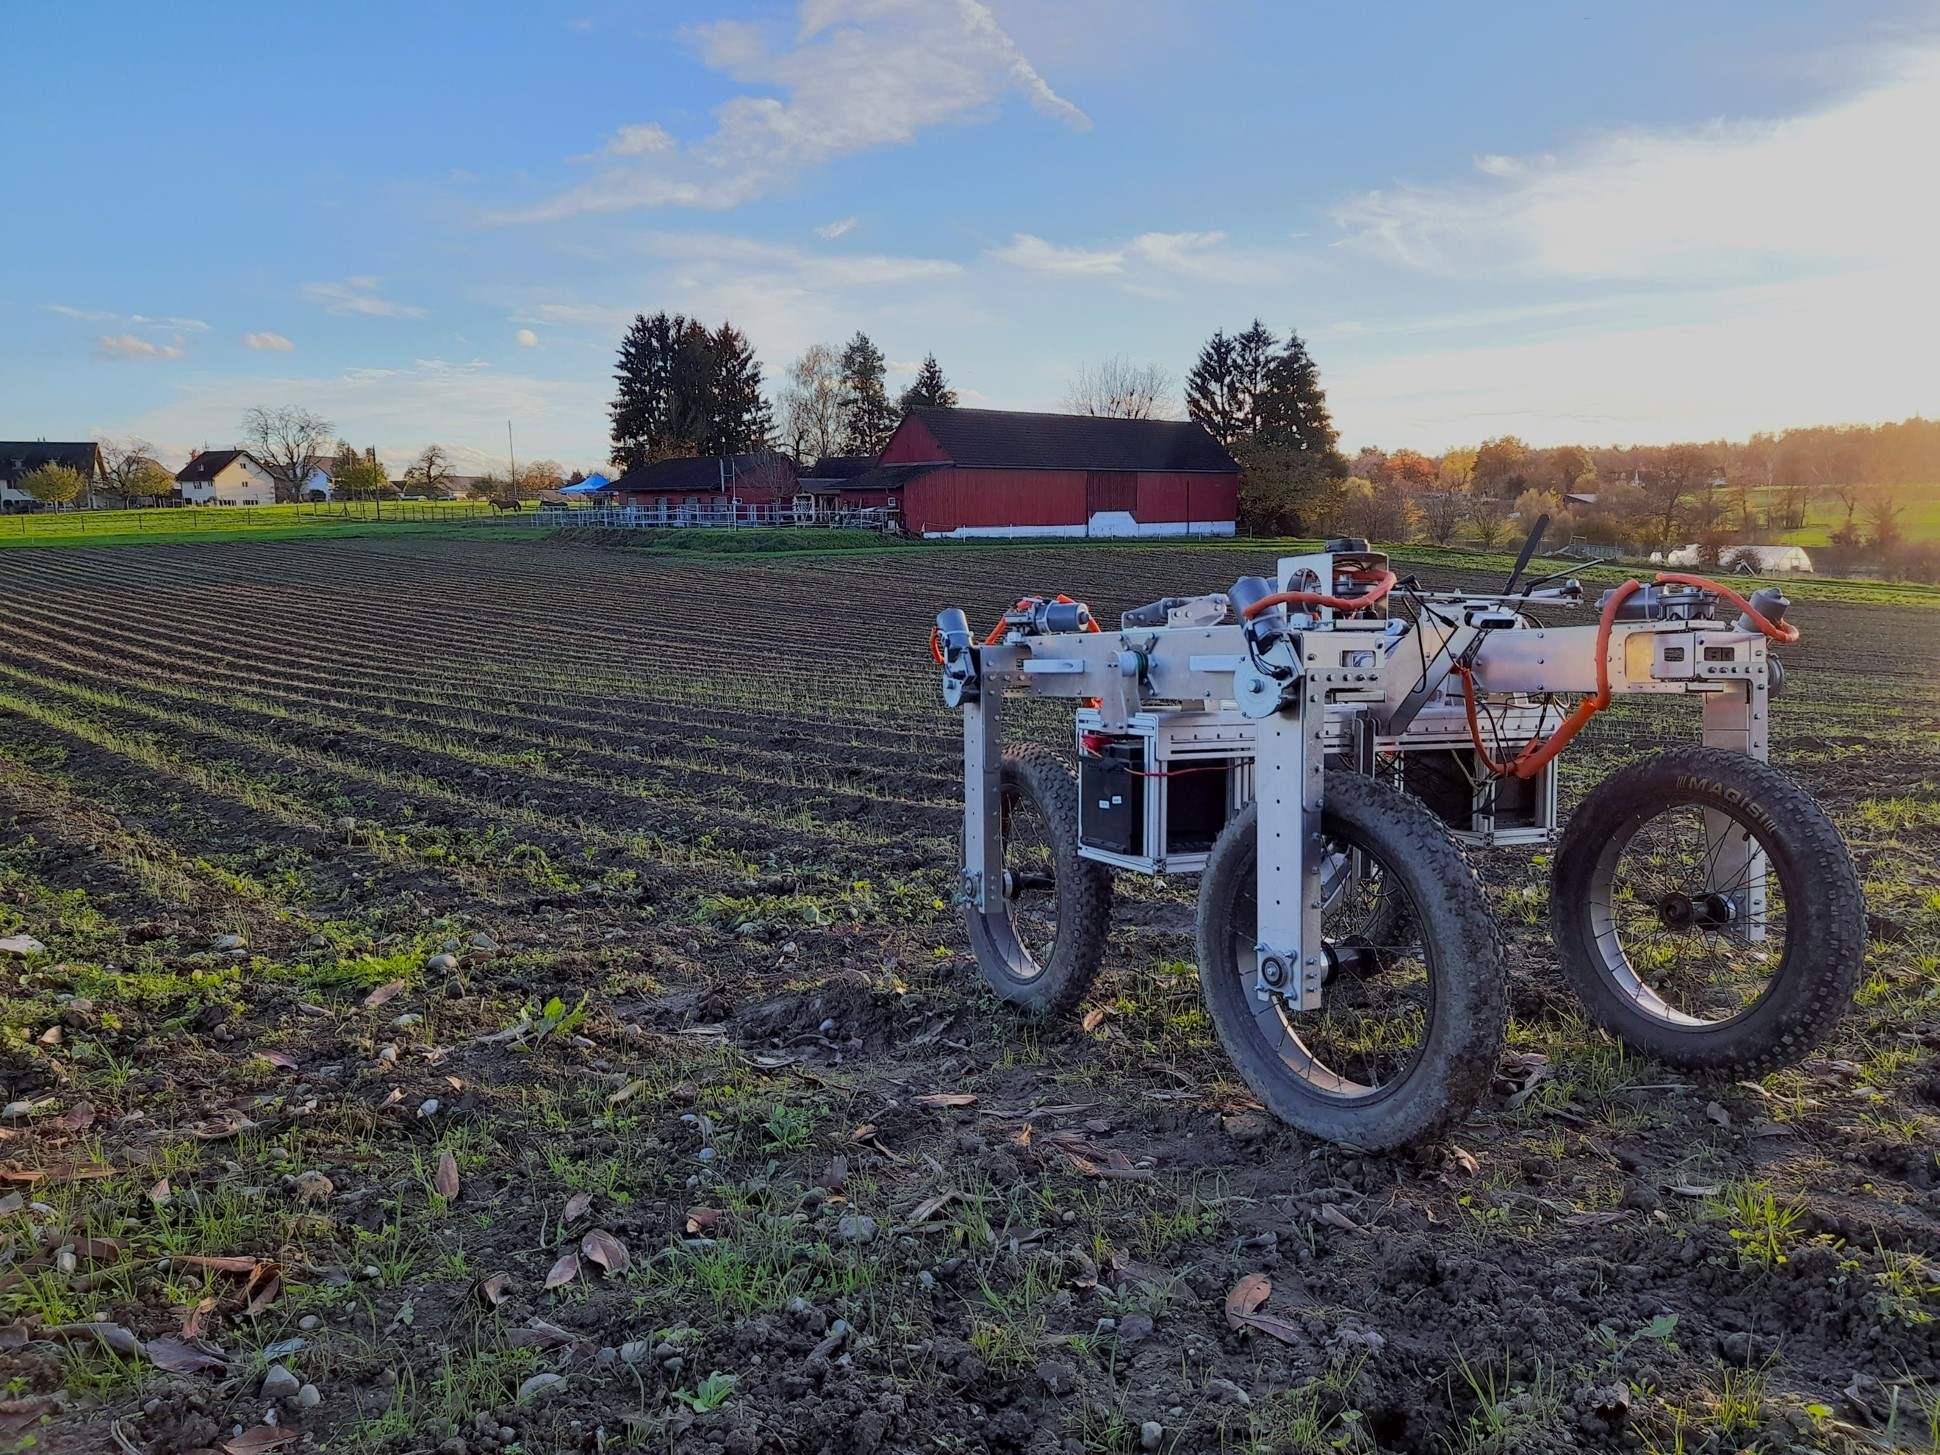
\includegraphics[width=0.75\textwidth]{Report/images/caterracoolrobot.jpg}
   \caption{Caterra's agricultural robot}
   \label{pics:coolrobot}
\end{figure}